\documentclass{article}
\usepackage[margin=0.8in]{geometry}
\usepackage{amssymb}
\usepackage{graphicx}

\title{Preface}
\author{by\\Donald Knuth \vspace{0.5in} \\Notes by Sriza}

\date{18th Feb, 2023}

\begin{document}
\maketitle
\thispagestyle{empty}
\newpage

\tableofcontents
\thispagestyle{empty}
\newpage

\section{Preface}
\setcounter{page}{1}
The process of preparing programs for a digital computer is especially attractive, not only because it is ecomically and scientifically rewarding, but also because it can be an aesthetic experience muct like composing poetry or music. The chapters in book are not meant to serve as an introduction to computer programming, the reader is supsposed to have had some previous experience. The reader should possess:
\begin{enumerate}
    \item Some idea of how a stored-program digital computer works(manner in which instructions can be kept in the machine's memory and successively executed.)
    \item An ability to put the solution to problems into such explicit terms that a computer can ``understand'' them.
    \item Some knowledge of most elementary computer techniques, such as looping, the use of subroutines and the use of indexed variables.
    \item A little knowledge of common computer jargon--``memory'', ``registers'', ``bits'', ``floating point'', ``overflow'', ``software''.
\end{enumerate}

This set of books is intended for people who will be more than just casually interested in computers, yet it is by no means only for the computer specialist. The main goal has been to make these programming techniques more accessible to the many people working in other fields who can make fruitful use of computers, yet who cannot afford the time to locate all the necessary information that is buried in technical journals. Knuths approach has been to try and distill the vast literature by studyint the techniques that are most basic, in the sencse that they can be applied to many type sof programming situations. He in this series has attempted to coordinate the ideas into more or less of a ``theory'', as well as to show hoew the theory applies to a wide variety of practical problems.

``Non numetical analysis'' is a terribly negative name for this field of study, and ``information processing'' is too broad a designation for the materials Knuth has considered, as well as ``programming techniques'' is too narrow. Therefore Knuth names the subject matter covered in this book as ``analysis of algorithm''.  This name is meant to imply ``the theory of the properties of particaular computer algorithms''.
\newpage

\section{General Outline}
The complete set of books, entitled The Art of Computer Programming, has the following general outline:
\begin{itemize}
    \item[] Volume 1. Fundamental Algorithms 
        \begin{itemize}
            \item[] Chapter 1. Basic Concepts
            \item[] Chapter 2. Information Structures
        \end{itemize}
    \item[] Volume 2. Seminumerical Algorithms 
        \begin{itemize}
            \item[] Chapter 3. Random Numbers
            \item[] Chapter 4. Arithmetic
        \end{itemize}    
    \item[] Volume 3. Sorting and Searching
        \begin{itemize}
            \item[] Chapter 5. Sorting
            \item[] Chapter 6. Searching
        \end{itemize}    
    \item[] Volume 4. Combinatorial Algorithms 
        \begin{itemize}
            \item[] Chapter 7. Combinatorial Searching
            \item[] Chapter 8. Recursion
        \end{itemize}
    \item[] Volume 5. Syntactical Algorithms
        \begin{itemize}
            \item[] Chapter 9. Lexical Scanning
            \item[] Chapter 10. Parsing
        \end{itemize}
\end{itemize}

Volume 4 deals with such a large topic, it actually represents three separate books ( Volumes 4A, 4B and 4C). Two additional volumes on more specialized topics are also planned: Volume 6, \textit{The Theory of Languages}; Volume 7, \textit{Compilers}. Knuth with these volumes tries to concentrate on ``classic'' techniques that are likely to remain important for many more decades. 

There are few words in order about the mathematical content of this set of books. These materials has been organized so that persons with no more than a knowledge of high-school algebra may read it, skimming briefly over the more mathematical portions. The knowledge of elementary calculus will suffice for most of the mathematics in this book. However, there is use of deeper theorems of complex variable theory, probability therory, number theory, etc., at times. The book uses machine-oriented language to specify computer algorithms due to following reasons:
\begin{enumerate}
    \item A programmer is greatly influenced by language in which programs are written. By underderstanding a machine-oriented language, the programmer will tend to use a much more efficient method.
    \item The programs we require are, with a few exceptions, all rather short, so with a suitable computer there will be no trouble understanding the program.
    \item High-level languages are inadequate for discussing important low-level details such as coroutine linkage, random number generation, multi=precision arithmetic, and many problems involving the efficient usuage of memory.
    \item A person who is more than casually interested in computers hsould be well schooled in machine language.
    \item New algebraic languages go in and out of fashion every five years or so.
\end{enumerate}

Given the decision to use a machine=oriented language, a question arises, which language should be used? Knuth here attempts to design an ``ideal'' computer with very simple rules of operation which resembles the actual machines very closely.

The best early papers are cited in the book, together with a sampling of more recent works. While referring to the literature, the standard abbreviations for the names of periodicals, except that the most commonly cited journals are abbreviated as follows:
\begin{enumerate}
    \item[] CACM = Communications of the Association for Computing Machinery 
    \item[] JACM = Journal of the Association for Computing Machinery 
    \item[] Comp. J. = The Computer Journal(British Computer Society)
    \item[] Math. Comp. = Mathematics of Computation 
    \item[] AMM = American Mathematical Monthly 
    \item[] SICOMP = SIAM Journal on Computing
    \item[] FOCS = IEEE Symposium on Foundations of Computer Science
    \item[] SODA = ACM-SIAM Symposium on FOundations of Computer Science
    \item[] STOC = ACM SYmposium on Theory of Computing
    \item[] Crelle =  Journal fur die reine and angewandte Mathematik
\end{enumerate}

As an example, ``CACM 6(1993), 555-563'' stands for the reference given in preceding paragraph of this preface. ``CMath'' stands for the book Concrete Mathematics.
\newpage

\section{Procedure for Reading this book}
\begin{enumerate}
    \item Begin reading this procedure, unless you have already begun to read it. \textit{Continue to follow the steps faithfully}
    \item Read the Notes on the exercises, on pages xv-xvii
    \item Set N equal to 1
    \item Begin reading Chapter N. Do not read the quotations that appear at the beginning of the chapter.
    \item Is the subject of the chapter interesting to you? If so, go to step 7; if not, go to step 6.
    \item Is N $\geq$ 2? If not, go to step 16; if so, scan through the chapter anyway. (Chapter 1 and 2 contain important introductory material and also a review of basic programming techniques, You should at least skim over the sections on notation and about MIX.)
    \item Begin reading the next section of the chapter; if you have already reached the end of the chapter, however, got to step 16.
    \item Is section number marked with ``*''? If so, you may omit this section on first reading (it covers a rather specialized topic that is interesting but not essential); go back to step 7.
    \item Are you mathematicall incliend? IF math is all Greek to you, got to step 11; otherwise proceed to step 10.
    \item Check the mathematical derivations made in this section(and report errors). Go to step 12.
    \item After you have worked on the exercises to your satisfaction, check your answers with the answer printed in the corresponding answer at the rear of the book. Also read the answers to the exercises you did not have time to work. Note: In most cases it is reasonable to read the answer to exercise n before working on exercise n+1, so steps 12-13 are usually done simultaneosly.
    \item Are you tired? If not, go back to step 7.
    \item Go to sleep. Then, wake up, and go back to step 7.
    \item Increase N by one. If N = 3,5,7,9,11, or 12, begin the next volume of this set of books.
    \item If N is less than or equal to 12, go back to step 4.
    \item Congratulations. Now try to get your friends to purchase a copy of Volume 1 and to start reading it. Also, go back to step 3.
\end{enumerate}

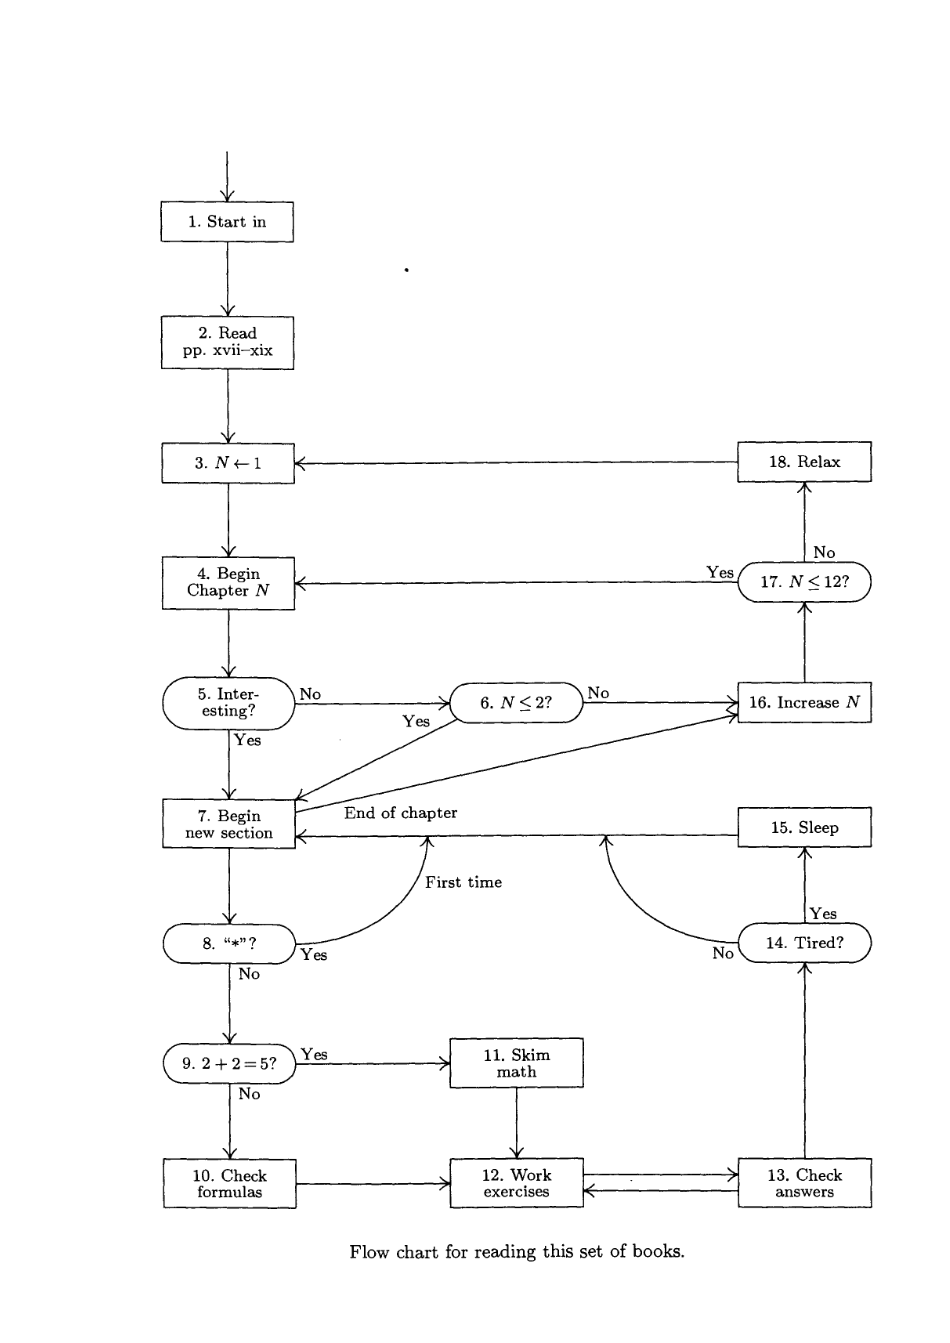
\includegraphics[width=0.9\linewidth]{./figs/fig_flowchart_for_reading_this_set_book.png}

\end{document}